\newpage
\chapter{A Clustering-Based Method for Automatic Educational Video Recommendation Using Deep Face-Features of Actors}
\label{chap:educational_recommendation}

It is a common practice among educational content creators to make collaborative videos, that is, videos in which more than one lecturer is presenting the lecture content.
%%
Such collaborations create a network of lecturers teaching a given subject.
%%
Therefore, a method that identifies these collaborations may help students find their content of interest more easily.
%%
In this chapter, we describe the second application we investigated using the \emph{Video Face Clustering} method.
%%
We propose a recommender method based on actor's presence for educational videos. In this case, the actors are lecturers~(or teachers, professors, etc.) that are presenting an educational content on video.
%%
For instance, if a student watches a video containing lecturers A and B, our method aims at recommending other videos that contain at least one of these lecturers. 
%%
This method provides an additional aid for educational recommender systems, allowing them to use the presence of lecturers as a feature for composing their recommendations.

The remainder of this chapter is structured as follows.
Section~\ref{sec:recommendation_dataset} presents the dataset we used.
We present our method in Section~\ref{sec:recommendation_method}, followed by 
Section~\ref{sec:recommendation_experiments}, that shows the experiments to validate the face clustering and the video recommendation ranking mechanisms.
Finally, in Section~\ref{sec:recommendation_discussion}, we conclude this chapter by discussing our results.

\section{Dataset}
\label{sec:recommendation_dataset}

The experiments were conducted using a dataset created in the context of this work.
It is composed of 98 educational videos publicly available on YouTube.\footnote{\url{https://www.youtube.com/channel/UCT0JugAtGmqiYkwxFZOwAtg}}$^{,}$\footnote{\url{https://www.youtube.com/user/deboraaladim}}
%%
Each video contains at least one lecturer; moreover, some videos could have some special participation or collaboration. Therefore, the number of lecturers in each video varies from 1 to 5. In total, 16 different lecturers are present in the dataset. Each lecturer is present, in average, in 6.67\% of the videos.
%%
We also annotated the name of each lecturer present in the videos, so that we can verify if correct videos are being recommended.

%%
The videos duration vary from 00m:30s to 1h:49m:01s. 
%%
The average duration of the videos is 23m:34s, with a standard deviation of 23m:05s. 
%%
The high value of the standard deviation for the time estimates indicates that the videos are not in the same time range, and therefore have a wide duration variety. 

\section{Proposed Method}
\label{sec:recommendation_method}

Our method intends to recommend educational videos based on the lecturers that appear in each video, so that, when a person watches a video, other videos containing the same lecturers are recommended.

For doing that, we first represent each video in the dataset of educational videos by the clusters of lecturers present using \emph{Video Face Clustering}. Once we have all videos represented, we perform the pipeline depicted in Figure \ref{fig:video_recommendation}. Each of the steps of this pipeline are described in the remainder of this section.

\begin{figure}[!ht]
  \centering
  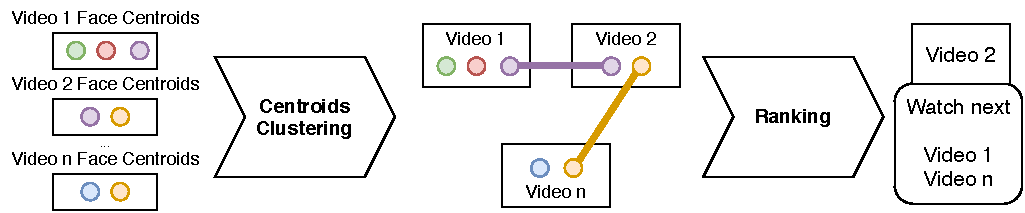
\includegraphics[width=1\textwidth]{img/video_recommendation/video_recommendation.pdf}
  \caption{Video Recommendation based on Lecturers Centroids Clustering}
  \label{fig:video_recommendation}
\end{figure}

First, we gather the centroids from the videos of the dataset as one single set and perform the \textit{Centroids Clustering}.
%%
For performing this clustering, we also use the strategy for an unknown number of clusters described in Algorithm \ref{clustering_alg}.
%%
By doing that, we group centroids from the same lecturer that are in different videos. For instance, in Fig. \ref{fig:video_recommendation}, one can see that the \emph{purple lecturer} is present in both Videos 1 and 2, while the \emph{orange lecturer} is present in both Videos 2 and n. By the end of this step, we have the group $L$ of lecturers present in the dataset of videos $V$. We also denote $L_v$ as the group of lecturers present in video $v$.

Next, based on these relationships among different videos, we perform \textit{Ranking}, by recommending videos in which lecturers of the current video are present. 
%%
For doing that, we compute a similarity score using the presence of the lecturers in the current video and the presence of these same lecturers in the other video.
%%
Let $p_{l,v}$ denote the percentage of frames in which the lecturer $l \in L_v$ is present in video $v \in V$. For each video $v \in V$ and $u \in V-v$ we compute a score of similarity $S_{v,u}$.

\begin{equation}
  S_{v,u} = \sum_{l~\in~L_v}{p_{l,v}\cdot{p_{l,u}}}
\end{equation}

Finally, using this score, for each video $v$ we compute a ranking $R_{v}$ where $R_{v,i}$ denotes the \emph{i-greatest} $S_v$ and $R_{v,i}\ge~R_{v,i+1}$ for all $i~\in~1...n_v$, where $n_v$ is the number of videos $u$ in which $S_{v,u}>~0$. 
%%
In this way, the more lecturers a video have in common with the reference video, and the more time these lecturers are present in both videos, the higher the video is positioned in the ranking of the reference video.  

By the end of this phase, we have a ranking of recommended videos for each video in the dataset.
%%
It is important to notice that our method is unsupervised and does not require the information of the lecturers in advance.
%%
Consequently, we do not store any information regarding the identity of the lecturers, respecting their privacy.


\section{Experiments}
\label{sec:recommendation_experiments}

\section{Discussion}
\label{sec:recommendation_discussion}